\chapter{Ocean models}
\lastupdated{2025-02-26}{\chapterFourOceanModOverleaf}

The modeling of the world's oceans for climate purposes is similar in many respects to the modeling of the atmosphere in terms of physical laws. However, there are key differences.
The oceans involve slower processes and larger-scale movements, and their motions are influenced by the shape of the bottom topography (ocean floor). Radiative fluxes in the ocean are also more complicated due to how light interacts with water. For climate, the most important ocean dynamics are the ones that occur on large scales and over long periods of time, the ones responding to low-frequency, large-scale processes, emphasizing the importance of long-term, broad patterns over short-term variability.
The time scales in the oceans are much longer than those in the atmosphere because of the greater thermal inertia; at the same time, the horizontal length scales are 1/10 of the atmosphere.

In the ocean, the hydrostatic approximation is an even better assumption. Furthermore, since sea water is nearly incompressible, the equation of continuity can be abbreviated by eliminating the time change of density, although density variations are generally included as far as buoyancy effects are concerned.

The Figure \ref{fig:equations in ocean dyn} shows the equation of the dynamics of the ocean.


\begin{figure}[h!]
	\centering
	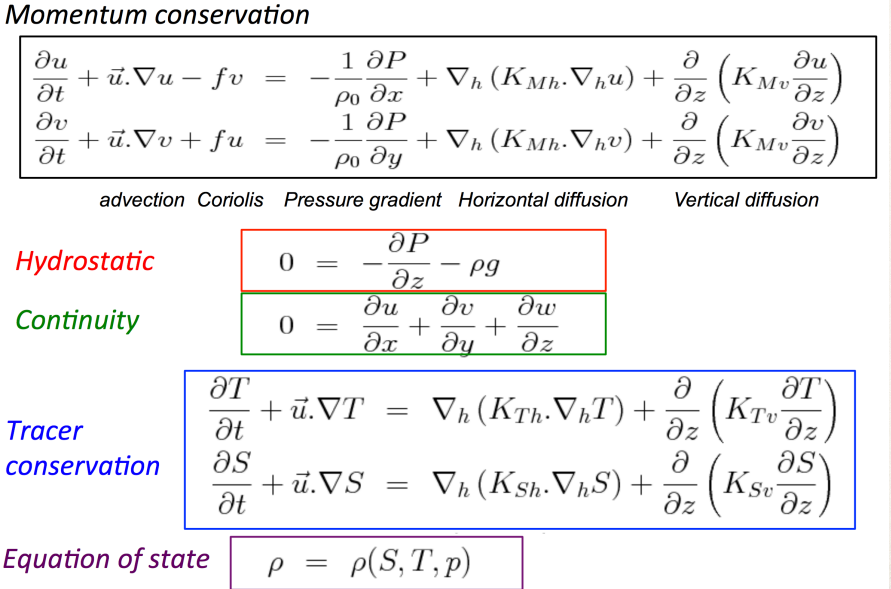
\includegraphics[width=0.4\linewidth]{upload/Screenshot 2024-11-21 225126.png}
	\caption{Equations in ocean dynamics}
	\label{fig:equations in ocean dyn}
\end{figure}
The equation of the state of the ocean is significantly different from the one of the atmosphere because it relates density to temperature, salinity, and pressure.
The frictional term for the atmosphere is replaced by vertical and horizontal viscous terms.
The hydrostatic equation is identical in form to that dor the atmosphere.
The first law of thermodynamics differs from that for the atmosphere because of the assumption of incompressibility, which allows the elimination of the term involving the time rate of change of density, and the replacement of the nonadiabatic term by explicit terms for the vertical and horizontal eddy diffusion of heat. \\


In addition, we have to take into consideration the fact that boundary conditions exist, like shown in Figure \ref{fig:boundary conditions}.
\begin{itemize}
	\item surface: upper level of the oceans in direct contact with the atmosphere (water can't go up surface of the ocean magically)
	\item bottom: assuming that there is no flux that goes into the bottom of the ocean
\end{itemize}


\begin{figure}[h!]


	\centering
	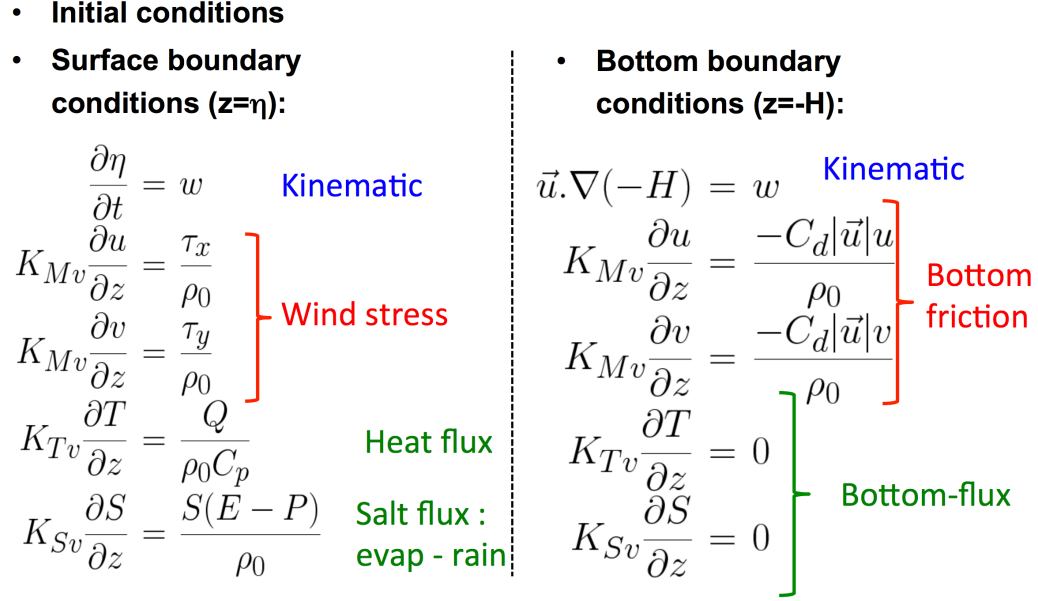
\includegraphics[width=0.5\linewidth]{upload/Screenshot 2024-11-21 225410.png}
	\caption{Boundary conditions}
	\label{fig:boundary conditions}
\end{figure}
At the bottom of the ocean $z=-H(\lambda,\phi)$, here there is zero stress and no vertical flux of sensible heat or salinity. The boundary conditions, at the bottom on the vertical motion, are such that the vertical motions here, are induced by horizontal motions interacting with the bottom topography.

Fluxes of temperature are also described due to the fact that cooling is more effective in mixing the oceans and that has an impact on ocean dynamics. Fluxes of salinity (due to evaporation and precipitation) are indicated because an increase of it causes an increase of density.\\



There are different ways by which the atmosphere can force the ocean.

\begin{itemize}
	\item transfer of momentum
	\item transfer of energy
	\item putting radiation fluxes on it
	\item evaporation - precipitation
\end{itemize}
For them, ocean response is related to the fact that if it is warm, it creates a pressure gradient and winds are created in response to it. \\




In 1969 Manabe and Bryan\cite{Manabe1969} investigated the calculus obtained with a combined ocean-atmosphere model. Their paper presented a model combining oceanic and atmospheric components, a pioneering step in simulating their interactions to study climate change and variability.  In their case, they are only allowed to use finite differencing and not spectral methods due to the boundary conditions. Some of the results are shown in Figure \ref{fig:result}; here we can see the difference between the average calculated in the model and the one observed: there is an error of 5 ° that nowadays would be unacceptable.


\begin{figure}[h!]
	\centering
	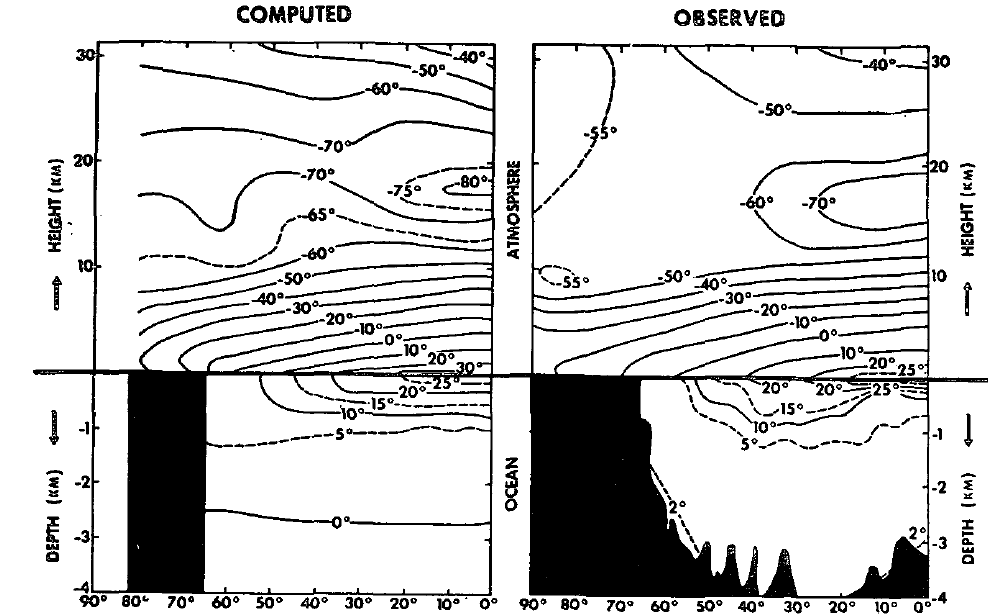
\includegraphics[width=0.5\linewidth]{upload/50image.png}
	\caption{left-hand side: zonal mean temperature of the system represents the time mean over two-sevenths of the period of the final stage of the time integration; right-hand side: observed distribution in the Northern Hemisphere}
	\label{fig:result}
\end{figure}

It is easy to see that the temperature increases until mid-latitude and after that it decreases, stressing the important difference between the surface and the deeper part in homogeneity.

Global ocean models often describe their horizontal
resolution with respect to their ability to permit or
resolve mesoscale (i.e. Rossby radius scale) eddies.

\paragraph{Problem with turbulence}
Turbulence is a complex phenomenon, and modeling it accurately is critical for understanding ocean circulation. Turbulence in the ocean involves processes like vertical mixing, eddies, and small-scale currents, that cannot be resolved explicitly. Turbulence must be parametrized, meaning its effects are approximately based on larger-scale variables resolved in the model. The closure problem of the turbulence refers to the difficulty of determining how unresolved turbulent processes interact with larger-scale dynamics. The challenge lies in creating a parameterization scheme that effectively captures the impact of turbulence on heat, momentum, and salinity transport. In their work, Manabe and Bryan employed simplifications for turbulent mixing, focusing on large-scale processes like thermohaline circulation, while acknowledging that small-scale turbulence was not fully resolved in their model.\\


The Manabe and Bryan model laid the foundation for modern coupled climate models. The challenges they identified, including the closure problem for turbulence, remain central to ocean modeling.
\begin{figure}[htpb]
	\centering
	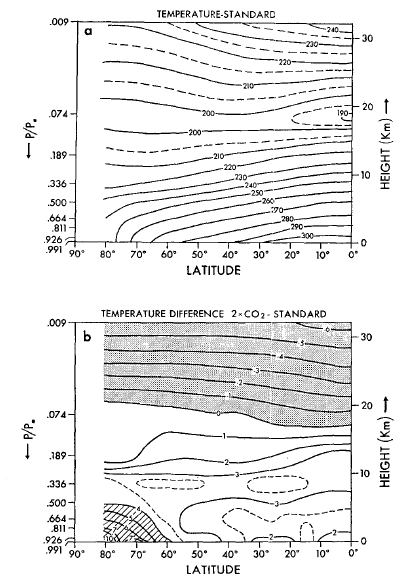
\includegraphics[width=0.3\linewidth]{upload/51image.png}
	\caption{Manabe and Wetherald 1975}
	\label{fig:fig 51}
\end{figure}


Manabe and Wetherald in 1975\cite{Manabe1975} tried to understand the effects of doubling $CO_2$ concentration on the climate of a General Circulation Model. The results yield some indication of how the increase of $CO_2$ concentration may affect the distribution of temperature in the atmosphere, in particular it raises in the troposphere and it lowers in the stratosphere (Figure \ref{fig:fig 51}).


\section{Ice models}

They are somewhat different from ocean models because they don't consider a fluid anymore but a solid, discontinuous in nature, varying in its distribution from one time period to another. In contrast to ocean and atmospheric models, whose calculations center on determining the properties of the water/air, with sea ice the primary goal is to determine the location and each time step, ice thickness and aerial ice concentration.



The calculation for climate-oriented sea ice models can be divided into two categories:

\begin{enumerate}
	\item calculations concerned with the thermodynamics of ice cover, the thickness and temperature structure of the ice, based on the principle of the conservation of energy.
	\item calculations concerned with the ice dynamic: determine the motion of the ice based on the conservation of momentum.
\end{enumerate}
(for more details on thermodynamics\&dynamics pag 129-146 book)

\section{The River Transport}

It is an important aspect of the hydrologic cycle, although it is often not incorporated into climate models. In the real world, the fresh water that flows in the ocean as continental runoff affects the ocean salinity, and thereby the ocean density and current structure, as well as forming a vital link in the water cycle of the climate system.\\




The water balance model is usually  part of the land vegetation surface component of the overall model and takes into account land cover type, monthly average of precipitation, potential evapotranspiration and temperature. Soil characteristics and topography are also inputs. Runoff has both surface and subsurface components. Eventually, the cumulative flow from the water transport model goes into the ocean.

\section{Grids}
Two possible grids: structured grids (cartesian, curvilinear) for global ocean, basin scale, coastal applications e.g. NEMO, MOM, ROMS, ecc; and unstructured grids, which domain is titled using more general geometrical shapes (triangles, ...) pieced together to optimally fit details of the geometry $\rightarrow$ tidal modelling, near shores, estuaries e.g. FVCOM, FESOM, MPAS, ecc.
\subsection{Regular grids}
\begin{itemize}
	\item regular spaced lines;
	\item on a spherical earth cannot have both uniform grid spacing and straight lines $\rightarrow$ grids tend to be curvilinear and the grid cell area tends to vary;
	\item lat-lon regular grids also have a problem at the poles where grid lines converge;
	\item they are computationally efficient;
	\item have a relatively straightforward analysis algorithm;
	\item have benefited from decades of research experience.
\end{itemize}
\textit{but} for a given latitude they have a fixed resolution: to increase resolution near the edge of an ocean basin (where you want it!) requires an increase of resolution everywhere including out in the middle of the ocean (where you don't!). An example are the tripolar grids: regular grid laid over the high latitude North Hemisphere region with two rotated poles located over land.
\paragraph{Unstructured grids}
\begin{itemize}
	\item irregular grids are designed to give more freedom to put spatial resolution where you want it
	\item a common scheme is composed as a series of triangles = finite elements
	\item by varying the size we can construct a non-uniform horizontal resolution over the computational domain
	      %this should be irregular grids??
	\item they are efficient owing to the fact that resolution can be tailored to need as a function of space
	\item they can accurately represent highly irregular coastlines and topography (no need fro "staircase" coasts and topography)
\end{itemize}
\textit{but} they have unresolved issues with flows dominated by geostrophy and advection (characteristics of large-scale ocean flows), and they have spacially variable resolution-dependent physics (e.g. viscosity and diffusivity coefficients should really be resolution dependent).

\paragraph{Adaptive Grids}
\begin{itemize}
	\item Unstructured meshes with a dynamically changing resolution responding to the nature of flow in time,
	\item they are very cool but very much in its infancy for ocean modeling applications.
\end{itemize}
\begin{figure}[htpb]
	\centering
	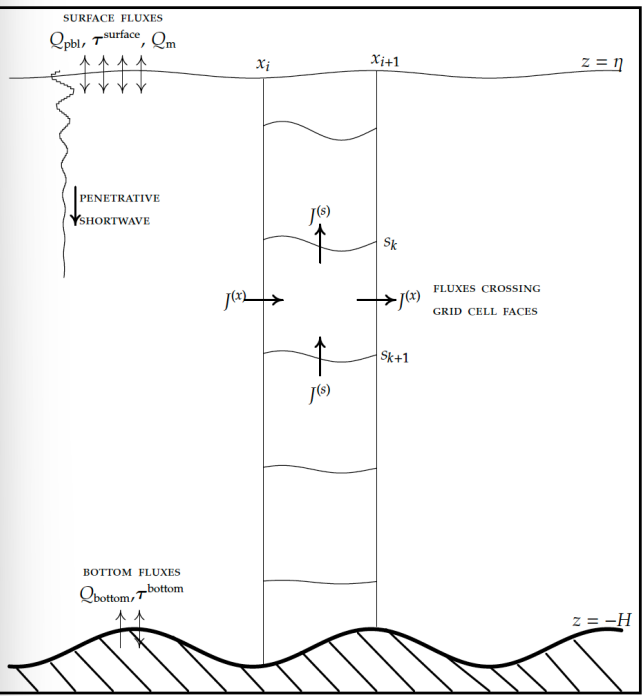
\includegraphics[width=0.4\linewidth]{upload/Screenshot 2024-11-21 235405.png}
	\caption{Vertical Grids}
	\label{fig:vertical grids}
\end{figure}
\paragraph{Vertical Grids}
The choice of the vertical coordinate system is loaded because:
\begin{itemize}
	\item the oceans are forced at the surface (most of the action occurs there);
	\item they are strongly stratified and they are adiabatic in the interior;
	\item there is complex bottom bathymetry to deal with.
\end{itemize}
As a consequence there exist a number of approaches to choose from. A different choice for the vertical coordinates can be done:
\begin{enumerate}
	\item Geopotential or Pressure: common for non-hydrostatic process modelling and large-scale climate modelling (\textcolor{Blue}{MITgcm},\textcolor{Blue}{MOM}, \textcolor{Blue}{NEMO})
	\item Isopycnal:  clean representation of interior quasi-adiabatic flows and overflows (\textcolor{Blue}{GOLD}, \textcolor{Blue}{HYCOM})
	\item Sigma: common for shelf/coastal modelling (\textcolor{Blue}{ROMS})
\end{enumerate}

\paragraph{Geopotential Coordinates}
Absolute depth/z-coordinate system. These are based on a serie of depth levels, it is common to add vertical resolution near the surface by decreasing the spacing between the levels in the upper ocean relative to the deep. Most common method for global models.
\begin{itemize}
	\item \textsc{advantages}: simple to set up, computationally efficient, there are no pressure gradient errors.
	\item \textsc{disadvantages}: increased vertical resolution near the lateral boundaries (i.e. continental slopes) requires the addition of grid cells throughout the basin; spurious diapycnal mixing associated with the numerical advection scheme.

\end{itemize}

\paragraph{Sigma} Terrain following or $\sigma$-coordinate system. It is based on the frational depth, scaled from 0 to 1: $0.01\sigma$ level is $1\%$ of the depth of the ocean, while $0.99\sigma$ level is at 99\% of the depth of the ocean. Applications for shelves and coastal areas.
\begin{itemize}
	\item \textsc{advantages}: mimics the bathymetry and allows high resolution near the sea floor regardless of depth or proximity to land.
	\item \textsc{disadvantages}: pressure gradient errors, issues with spurious diapycnal mixing coming from the numerical advection scheme
\end{itemize}

\paragraph{Isopycnal vertical coordinates} Density ($\rho$)/"layered models". The vertical grid is defined by density surfaces, it exploits the fact that below the mixed layer, ocean currents generally flow along surfaces of equal density (flow is "adiabatic").
\begin{itemize}
	\item \textsc{advantages}: simple, "exactly isopycnal"
	\item \textsc{disadvantages}: perform poorly where the ocean is less stratified (e.g. in shallow water); no resolution in an unstratified fluid; no mixed layer unless you tack one on; issues with entrainment.
\end{itemize}
\begin{figure}[htp!]
	\centering
	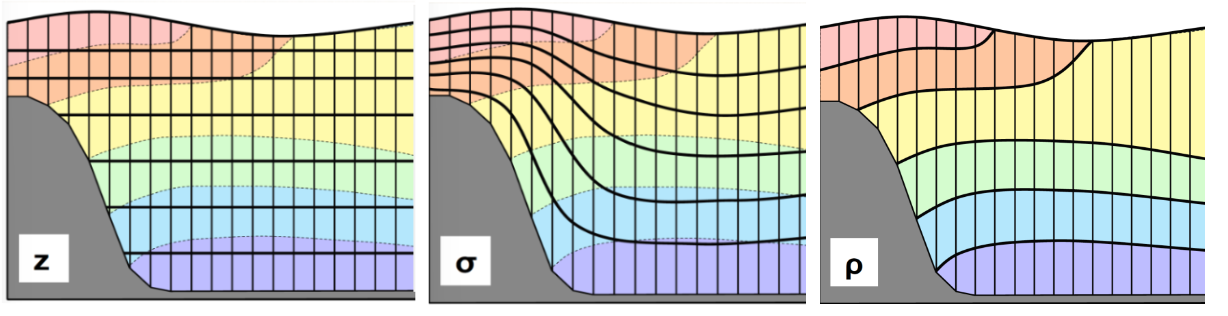
\includegraphics[width=0.5\linewidth]{upload/Screenshot 2024-11-22 001323.png}
	\caption{$z$, $\sigma$ and isopycnal coordinate systems}

\end{figure}
\paragraph{Hybrid coordinates} It seeks to optimize performance by combining the best suited system in different regions based on the dominant processes at work. HYCOM=z coordinates in the surface mixed layer and density coordinates in the stratified ocean below. Here the vertical coordinates evolve in both time and space as the depth of the mixed layer changes.
\begin{itemize}
	\item \textsc{advantages}: dynamically optimized coordinate system gives improved results.
	\item\textsc{disadvantages}: high computational costs.
\end{itemize}

\begin{figure}[htp!]
	\centering
	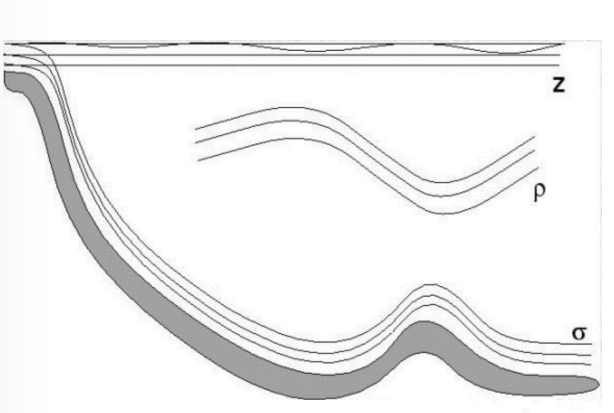
\includegraphics[width=0.2\linewidth]{upload/Screenshot 2024-11-22 000943.png}
	\caption{Hybrid coordinates}

\end{figure}
\subsection{Resolution and mesoscale eddies}
\begin{center}
	"Eddy-resolving" at 1/10° is not enough to resolve ocean "weather"
\end{center}
\textbf{\textcolor{Blue}{Eddies} are swirling, circular movements of water in the ocean}, resembling whirlpools, but they can vary greatly in size and duration. They are a fundamental aspect of ocean dynamics, transporting heat, nutrients, salt, and momentum across the ocean. Eddies often form due to \textbf{shear instabilities (differences in velocity between layers), boundary currents (for instance Gulf Stream) and topography}.
The horizontal resolution needed to resolve the first barolinic deformation radius with two grid points.
\begin{itemize}
	\item[$\blacksquare$] There are different rules of thumb. One is that it takes 5 grid points to accurately define a feature without aliasing: this means 1/8° global resolution ($\sim$ 15 km) can accurately depict only features larger than $\sim$ 60 km;
	\item[$\blacksquare$] Models with variable grid spacing have variable resolution - beware of resolution dependent physics!
	\item[$\blacksquare$] Resolution is not cheap - because of the CFL\footnote{Courant–Friedrichs–Lewy stability condition} (NB. no transport faster than one grid cell per time step) condition, as we shrink the horizontal grid spacing we must add vertical layers and decrease the time step
\end{itemize}
At all (present-day) resolution, OGCMs resolve the mesoscale in some regions but not others. \\



Global ocean models often describe their horizontal resolution with respect to their ability to permit or resolve mesoscale (i.e. Rossby radius scale) eddies.
Eddy-resolving does NOT mean all eddies are resolved or that all eddy effects of resolved eddies are acting. The spatial resolution of the ocean component of CMIP5/CMIP6\footnote{see chapter \ref{chapter7}} coupled models is 0.2° to 2°/0.1° to 1°: from coarse (no eddies) to eddy-permitting (partially resolved eddy field). The effects of eddies need to be parameterized in coarse models (more later!); what to do in models that partially resolve the eddy field is an increasingly important question.
\begin{figure}[htpb]
	\centering
	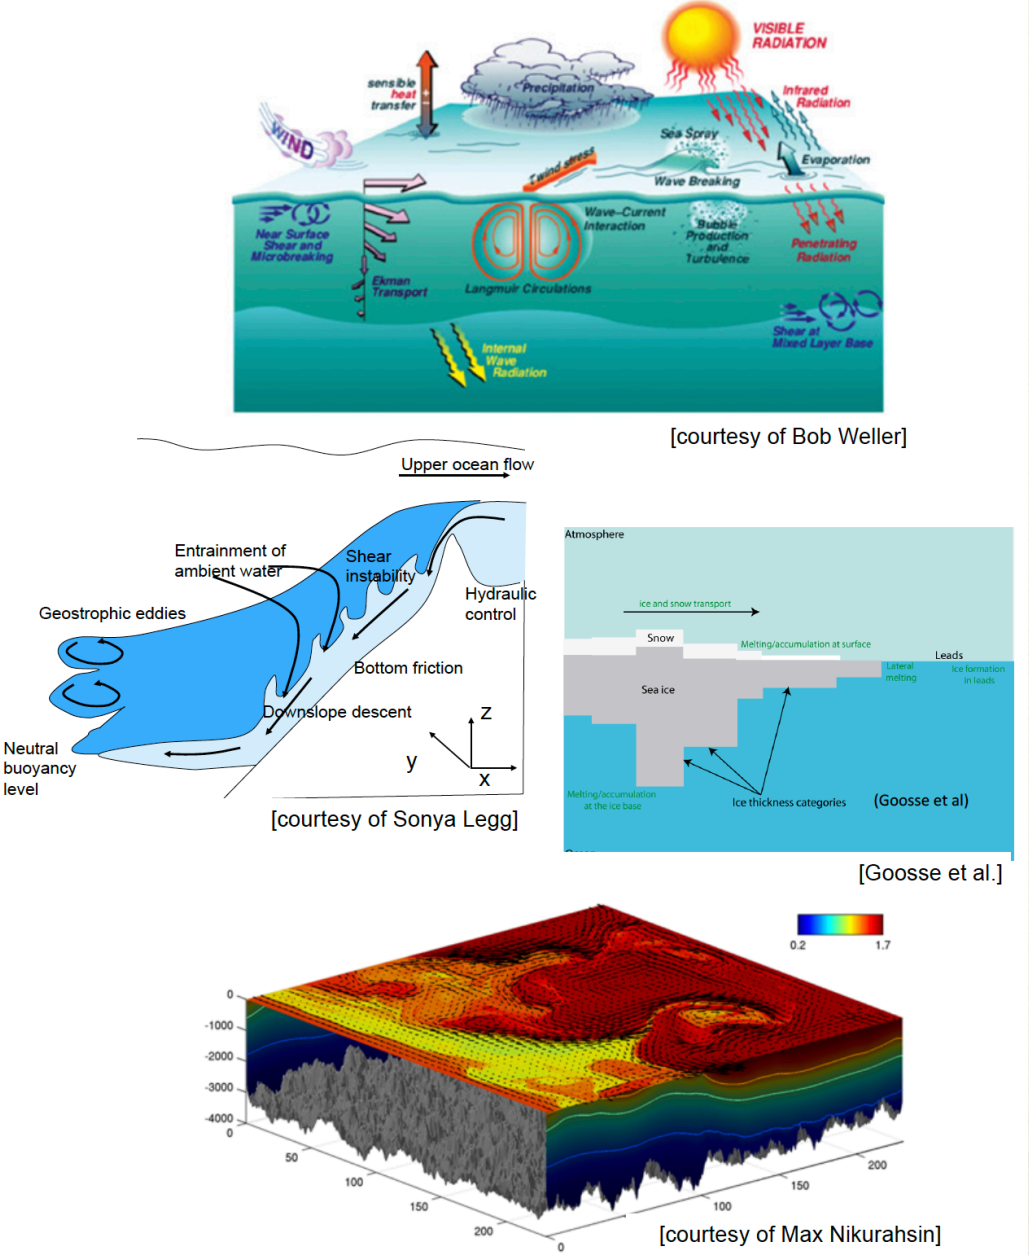
\includegraphics[width=0.35\linewidth]{upload/Screenshot 2024-11-22 104603.png}\quad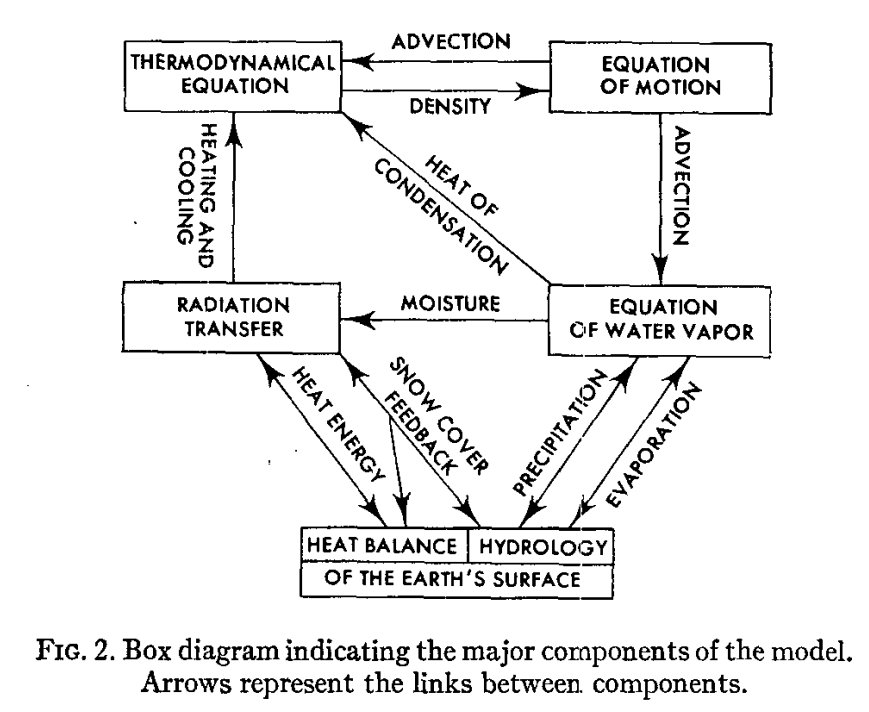
\includegraphics[width=0.35\linewidth]{upload/Screenshot 2024-11-24 185214.png}
	\caption{Fig.a: Parametrization and eddie problems. Fig.b: Major components of the model}
	\label{...}
\end{figure}
\subsubsection{Parametrizations}
Processes need to be parametrized in a model for two reasons:
\begin{enumerate}
	\item we don't spend the computational resources required to directly treat them because they are either too small or too complex.
	\item we don't understand it well enough to be represented by an equation
\end{enumerate}
Processes commonly parametrized in ocean models include: mesoscale eddy effects - submesoscale eddy effects - dense
overflows - coastal processes - surface mixed layer processes
- friction - sub-grid scale mixing - ocean-ice interactions.
\begin{itemize}
	\item[] \textit{low resolution models}: the main problem is mesoscale eddies
	\item[] \textit{high resolution models}: submesoscale eddies (fronts and filaments), internal wave mixing, details of flowtopography interactions.
\end{itemize}

\subsubsection{Kind of eddies}
The models must reproduce the eddy transport properties well otherwise that cannot maintain the basic flow.
\paragraph{Blackmon 1976}\cite{M.L.Blackmon1976}  used spectral methods to decompose the variability of the 500 mbar geopotential height field into different spatial and temporal scales. He found:
\begin{itemize}
	\item \textbf{Low-Frequency Variability (Planetary Waves):} Highlighted the dominance of quasi-stationary planetary-scale waves (large-scale undulations in the jet stream).
	\item \textbf{High-Frequency Variability (Synoptic Waves):} Identified transient synoptic-scale systems (e.g., midlatitude cyclones and anticyclones) as major contributors to the atmospheric variability.
\end{itemize}
He demonstrated that most of the variability occurs at intermediate (synoptic) scales. He quantified the distribution of energy across scales, helping to clarify the relative importance of large-scale versus small-scale atmospheric processes. He also found significant geographical differences in the distribution of wave activity, with distinct patterns in storm tracks over the Northern Hemisphere.

\paragraph{Bjerknes} Jacob Bjerknes, the son of renowned meteorologist Vilhelm Bjerknes, is celebrated for his groundbreaking work in linking El Niño to the Southern Oscillation during the 1960s. While already recognized for his earlier contributions to the theoretical cyclone model developed with the "Bergen School" in the 1920s, Bjerknes turned his attention to understanding the dynamics of the equatorial Pacific.

Bjerknes observed that the sea surface temperatures (SSTs) in the eastern Pacific were unusually cold for such low latitudes, creating a sharp temperature contrast with the warm waters of the western Pacific. This temperature gradient drives a distinct atmospheric circulation, with cool, dry air moving westward along the surface and rising as warm, moist air in the western Pacific. Bjerknes named this systematic east-west atmospheric flow the Walker Circulation (see chapter \ref{chapter1} for more info).

He proposed that fluctuations in the Walker Circulation could trigger changes in the Southern Oscillation, setting off events associated with El Niño-Southern Oscillation (ENSO). Bjerknes described a feedback loop in which stronger easterly winds enhanced the upwelling of cold water in the east, intensifying the SST gradient and reinforcing the Walker Circulation. Conversely, weaker easterly winds reduced upwelling, diminished the SST gradient, and slowed the circulation. This mechanism explained the alternation between the warm El Niño phase, marked by a weakened Walker Circulation, and the normal cold state of the eastern Pacific associated with the high phase of the Southern Oscillation.

Bjerknes’ insights established the foundation for modern understanding of ENSO, demonstrating how oceanic and atmospheric systems interact in a dynamic feedback loop to shape global climate patterns.
\begin{figure}[htpb]
	\centering
	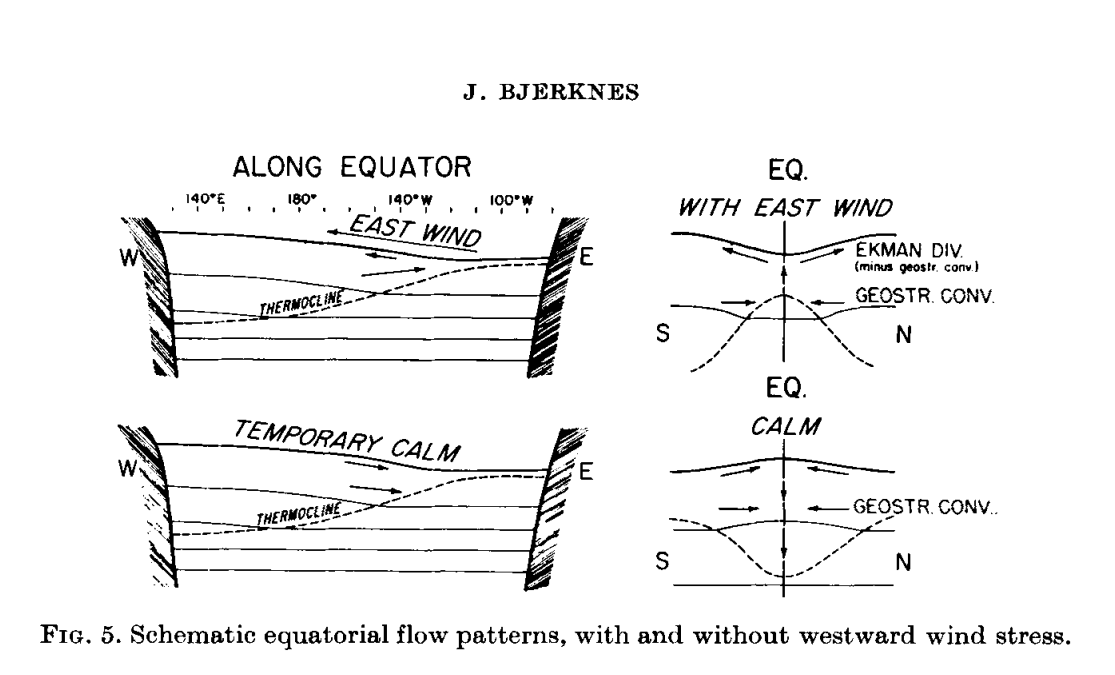
\includegraphics[width=0.35\linewidth]{upload/Screenshot 2024-11-24 191635.png}
	\caption{The Walker Circulation}

\end{figure}
The Walker Circulation is driven by the east-west SST gradient along the equatorial Pacific: warm SSTs in the western Pacific generate low-pressure systems, promoting rising air and convection (clouds and rainfall); cool SSTs in the eastern Pacific lead to high-pressure systems, with descending air and dry conditions.
This SST gradient establishes the pressure differences necessary for the Walker Circulation, with surface easterly winds flowing westward and upper-level winds returning eastward: stronger SST gradients reinforce the Walker Circulation by intensifying convection in the west and upwelling in the east. Weaker SST gradients, such as during El Niño events, disrupt the Walker Circulation by reducing pressure differences, weakening trade winds, and allowing warm water to spread eastward.

Climate forcing (e.g. global warming) modifies SST patterns, disrupting or enhancing the Walker Circulation. Changes in the Walker Circulation, in turn, influence SST distributions and climate change.
\section{Caos}
It is actually a misnomer, we should really talk about “sensitivity to initial conditions” (\cite{Tanner2020}).
The idea had been fluctuated for some time both in Maxwell and Poincare’ work, probably the first colourful image was done by WS Franklin (1898). Ed Lorenz (1972) after seminal works in 1963 and 1969 introduced in 1972 at 139th Meeting of the AAAS, the concept ‘Does the flap of a buttery’s wings in Brazil set off a tornado in Texas?’.
Deterministic ideas dating to Newton and hyperdeterministic ideas by PS Laplace were put in discussion.
\paragraph{Lorenz System}
\begin{align}\label{eq.lorenz system}
	\frac{dx}{dt}=\sigma(y-x) \\
	\frac{dy}{dt}=x(\rho-z)-y \\
	\frac{dz}{dt}=xy-\beta z
\end{align}
The solutions of this system represent the traveling waves around a cycle of constant latitude.
\begin{align*}
	\dot{x_j}=x_{j-1}(x_{j+1}-x_{j-2})-x_j+F \quad \text{for} \quad j=1,\dots,N \\
	x_{j-N}=x_{j+N}=x_j
\end{align*}
\section{Vorticity dynamics}
\subsection{What maintains the circulation?} Starting from the basic structure of the wind, the jet is the factor maintaining the circulation. We need to write the equations of the jet stream. Consider the vorticity budget for a non-divergent case:
\begin{equation}
	\frac{\partial\zeta}{\partial t}=-\vec{v}\cdot\nabla(\zeta+f)
\end{equation}
and introduce now the zonal mean:
\begin{equation}\label{eq.zonal mean}
	\overline{A}=\frac{1}{2\pi}\int_0^{2\pi}Ad\lambda
\end{equation}
separate each field in zonal mean and deviation, $A=\overline{A}+A'$:
$$\frac{\partial}{\partial t}(\overline{\zeta}+\zeta')=-(\overline{u}+u')\frac{\partial}{\partial x}(\overline{\zeta}+\zeta')-(\overline{v}+v')\frac{\partial}{\partial y}(\overline{\zeta}+\zeta'+f_0+\beta y)$$
because it is tangent to the Earth and it needs linearization, zonally averaging again:
\begin{equation}\label{eq.average eq}
	\frac{\partial\overline{\zeta}}{\partial t}=-\overline{u}\frac{
		\partial\overline{\zeta}
	}{\partial x}-\overline{v}\frac{\partial\overline{\zeta}}{\partial y}-\beta \overline{v}-\frac{\partial}{\partial y}\overline{v'\zeta'}
\end{equation}
because $\overline{A}=0$, subtracting this equation from the first we get an equation for the perturbation. Notice that because in the non-divergent case there exists a streamfunction, then $v=\psi_x$ so $\overline{v}=0$ for the periodic boundary conditions:
$$\frac{\partial\zeta'}{\partial t}=-\overline{u}\frac{\partial\zeta'}{\partial x}-v'\frac{\partial\overline{\zeta}}{\partial y}-\beta v'-\frac{\partial}{\partial x}(u'\zeta')-\frac{\partial}{\partial y}(v'\zeta'-\overline{v'\zeta'})$$ for small perturbation we can linearize it:
\begin{equation}
	\frac{\partial\zeta'}{\partial t}=-\overline{u}\frac{\partial\zeta'}{\partial x}-v'\frac{\partial\overline{\zeta}}{\partial y}-\beta v'
\end{equation}
consider the mean equation \ref{eq.average eq}, $\overline{\zeta}=\overline{v}_x-\overline{u}_y$, but the zonal mean of a total derivative in $x$ is zero because of periodic boundary conditions, so $\overline{\zeta}=-\overline{u}_y$:
$$-\frac{\partial}{\partial y}\frac{\partial\overline{u}}{\partial t}=-\overline{u}\frac{\partial\overline{\zeta}}{\partial x}-\overline{v}\frac{\partial\overline{\zeta}}{\partial y}-\beta\overline{v}-\frac{\partial}{\partial y}\overline{v'\zeta'}$$
because it is not divergent, the mean meridional flow can be obtained from a streamfunction, $v=\psi_{x'}\overline{v}$ is also zero, then
$$-\frac{\partial}{\partial y}\frac{\partial\overline{u}}{\partial t}=+\overline{u}\frac{\partial}{\partial x}\frac{\partial\overline{u}}{\partial y}-\frac{\partial}{\partial y}\overline{v'\zeta'}$$
averaging again and remembering that the $x$-derivative of a zonally averages quantity is zero we get:
\begin{align*}
	\frac{\partial\overline{u}}{\partial t}=\overline{v'\zeta'} \\
	\frac{\partial\overline{u}}{\partial t}=-\frac{\partial}{\partial y}\overline{v'u'}
\end{align*}
This relation shows that the acceleration of the mean flow is caused by the meridional fluxes of momentum. A similar relation can be found for the mean zonal temperature linked to the eddy heat flux.


The relation between eddies and jet streams holds also in the three-dimensional case in the quasi-geostrophic approximation. In this case however we have also non zero
zonal meridional and vertical velocity $(v,w)$.
$$\frac{\partial\overline{u}}{\partial t}=f_0\overline{v}-\frac{\partial}{\partial y}\overline{v'u'}$$
we can then find similar relations for the zonal mean of the temperature:
\begin{equation}\label{eq.zonal mean of temperature}
	\frac{\partial\overline{\theta}}{\partial t}=-N^2\overline{w}-\frac{\partial}{\partial y}\overline{v'\theta'}
\end{equation}
The thermal wind relations link the variables:
\begin{align}\label{eq.thermal wind}
	f_0\frac{\partial\overline{u}}{\partial z}=-\frac{\partial\overline{\theta}}{\partial y} \\
	\frac{\partial\overline{v}}{\partial y}=-\frac{\partial\overline{w}}{\partial z}
\end{align}
\begin{figure}[htpb]
	\centering
	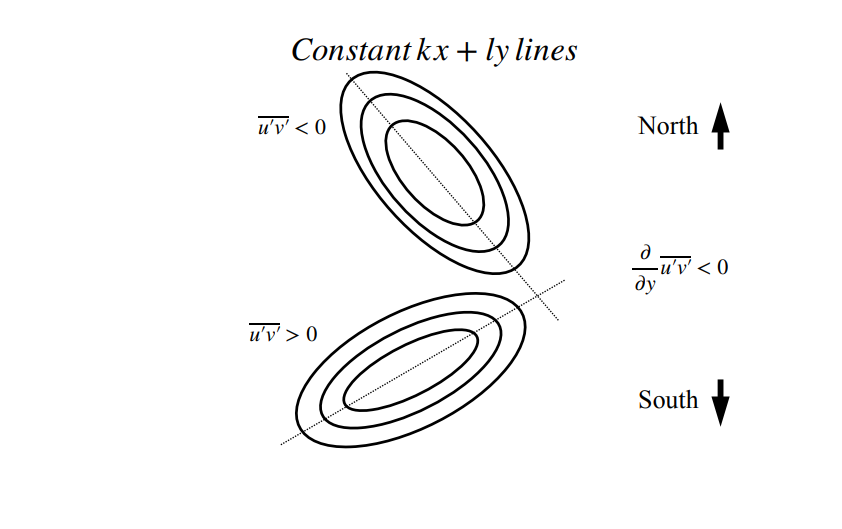
\includegraphics[width=0.35\linewidth]{upload/Screenshot 2024-11-22 202457.png}\quad 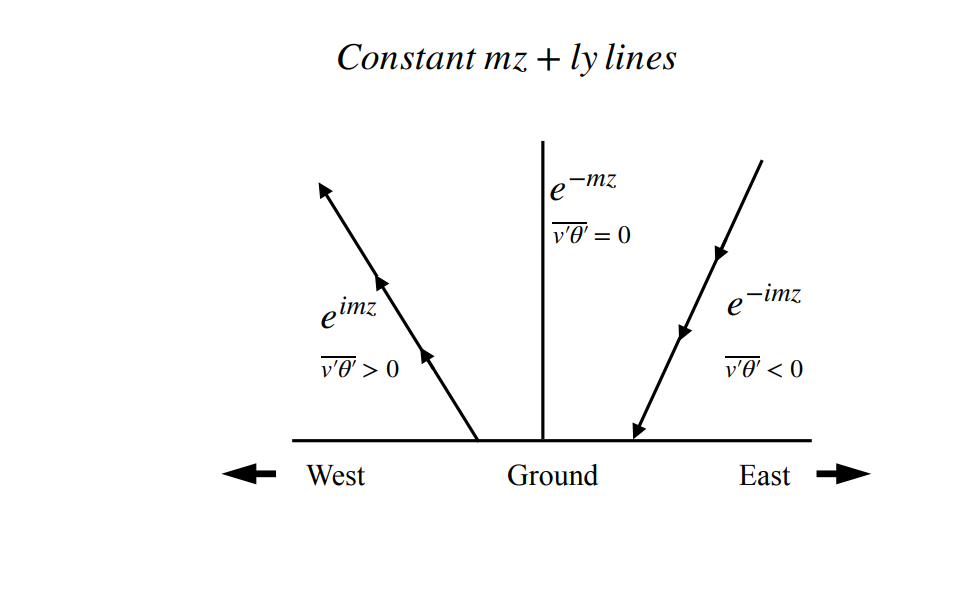
\includegraphics[width=0.35\linewidth]{upload/Screenshot 2024-11-24 185505.png}
	\caption{a) Momentum Flux. The meridional transport of momentum depends on the meridional slant of the eddies. b) Heat flux. The meridional transport of heat depends on the vertical slant of the eddies.}

\end{figure}
